\documentclass[conference]{IEEEtran}

\usepackage{pifont}
\usepackage{graphicx}
\usepackage{amsmath}
\usepackage{mybeamer}
\usepackage{draftwatermark}

\begin{document}

\title{Flow Specification in GEM5}

\maketitle


\begin{abstract}
This paper will go through a brief overview for the implemented instances of these flows are given. These flow specifications capture how messages are exchanged for different use cases. In this model, a message is defined with the following format, (Src,Dest,Cmd), where Src and Dest refer to the source and destination components of messages, Cmd refers to the operations that the destination component should perform. 
\end{abstract}



\section{write flow specification}


 \begin{figure} 
 \centerline{
 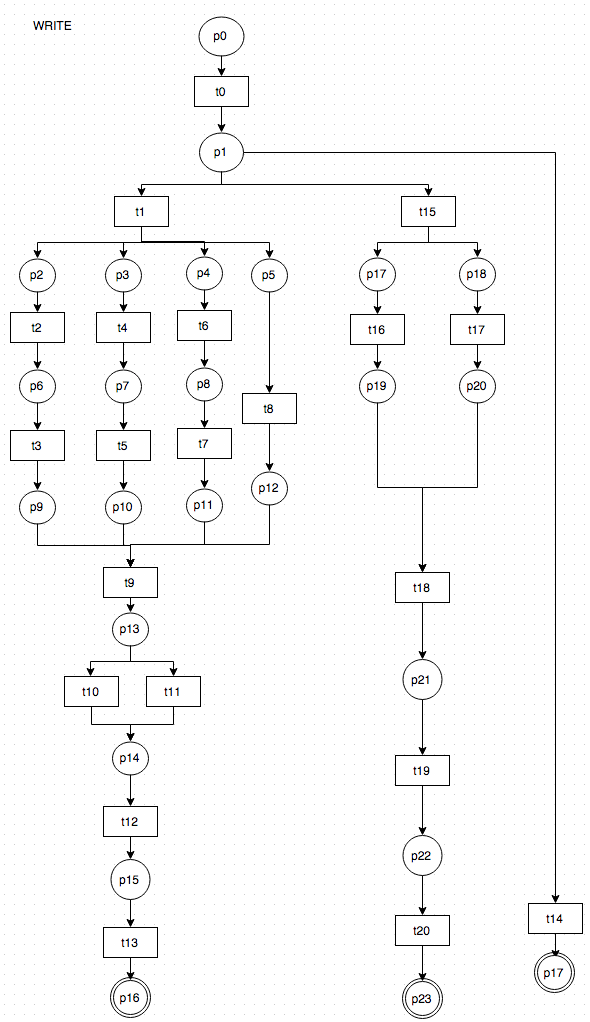
\includegraphics[width=3.4In]{figures/Fig5.png}}
 
 {\footnotesize
 \[
 \begin{array}{llll}
 msg_0: (&\mbox{ CPU1},&\mbox{writeReq},&\mbox{icache1   })\\       
 msg_1: (&\mbox{ dcache1},&\mbox{ readExreq },&\mbox{Bus     })\\        
 msg_2: (&\mbox{ Bus},&\mbox{ readExreq},&\mbox{ dcahce2 })\\  
 msg_3: (&\mbox{ dcache2},&\mbox{readExreq},&\mbox{cpu2         })\\   
 msg_4: (&\mbox{ Bus},&\mbox{ readExreq},&\mbox{ icahce2           })\\  
 msg_5: (&\mbox{ icache2},&\mbox{readExreq},&\mbox{cpu2 })\\  
 msg_6: (&\mbox{ Bus},&\mbox{ readExreq},&\mbox{ icahce1       })\\     
 msg_7: (&\mbox{ dcache1},&\mbox{readExreq},&\mbox{cpu1           })\\  
 msg_8: (&\mbox{ Bus},&\mbox{ readExreq},&\mbox{ Memory })\\  
 msg_9: (&\mbox{ true                                          })\\  
 msg_{10}: (&\mbox{ Memory},&\mbox{ readExres},&\mbox{ Bus        })\\  
 msg_{11}: (&\mbox{ icache2},&\mbox{ readExres},&\mbox{ Bus })\\  
 msg_{12}: (&\mbox{ Bus},&\mbox{ readExres},&\mbox{ dcache1        })\\  
 msg_{13}: (&\mbox{ icache1},&\mbox{ writeRes},&\mbox{ CPU1         })\\  
 msg_{14}: (&\mbox{ icache1},&\mbox{ writeRes},&\mbox{ CPU1 })\\  
 msg_{15}: (&\mbox{ dcache1},&\mbox{UpgradeReq             })\\  
 msg_{16}: (&\mbox{ Bus},&\mbox{ UpgradeReq},&\mbox{ icahce2      })\\   
 msg_{17}: (&\mbox{ Bus},&\mbox{ UpgradeReq},&\mbox{ Memory })\\  
 msg_{18}: (&\mbox{ icache2},&\mbox{UpgradeRes},&\mbox{ Bus     })\\  
 msg_{19}: (&\mbox{ Bus},&\mbox{ UpgradeRes},&\mbox{ icache1      })\\  
 msg_{20}: (&\mbox{ icache1},&\mbox{ WriteRes},&\mbox{ CPU1 })\\  
 \end{array}
 \]}
 \caption{Flow specification ($F_1$) of a cache coherent write operation initiated from CPU1}
 \label{write-flow}
 \end{figure}
 
 The LPN as shown in Fig.~\ref{write-flow} specifies a system flow where CPU1 initiates a memory write operation. In this flow, CPU1 initiates a memory write request to L1 Cache. Next, depends on whether the required data is included in cache1, the cache1 will generate three possible responses. First, the cache1 will send read exclusive request message msg2 to interconnect if data is not present in cache; Or if the data is shared by CPU0, it will send upgrade message msg16 to interconnect to disable CPU0's ownership of this block of data, else if CPU1 has exclusive right of required data, cache1 will perform the write operation and sent an response message msg15 to CPU1. Afterwards, interconnect will sent request to all connected component (data cache and instruction cache of each CPU and memory). Once the interconnect obtains the response from either CPU0 or memory, it will generate a response message to cache1, then cache1 will generate a write response message msg14 (or msg 21 ) to CPU1. The flow is symmetric for CPU2.
 
 
 
 \section{read flow specification}
 
 \begin{figure} 
 \centerline{
 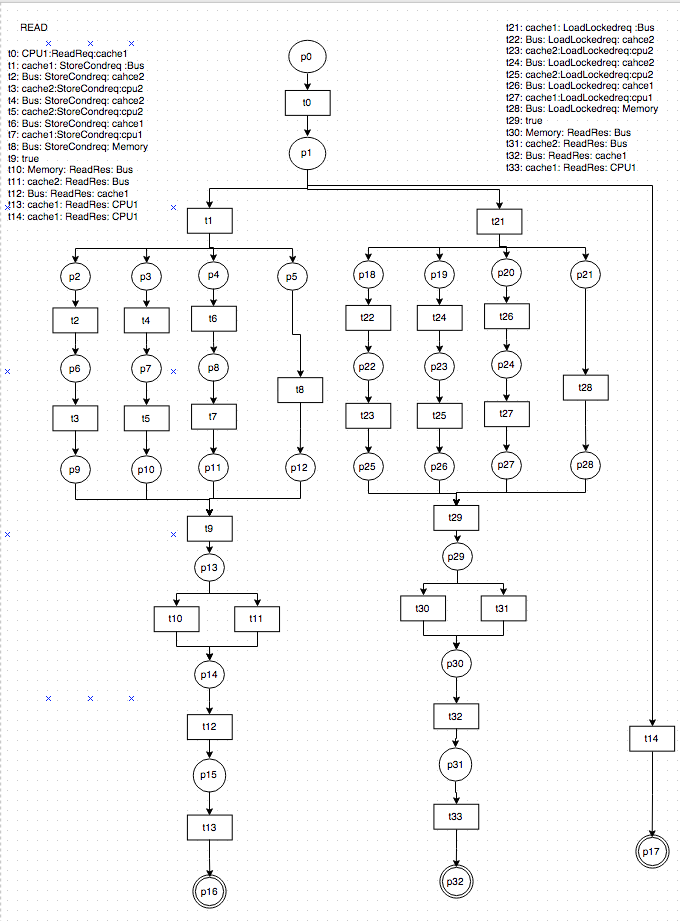
\includegraphics[width=3.33in]{figures/Fih6.png}}
 
 {\footnotesize
 \[
 \begin{array}{llll}
 msg0: (&\mbox{ CPU1},&\mbox{ReadReq},&\mbox{icache1  })\\                   
 msg1: (&\mbox{ dcache1},&\mbox{ StoreCondreq },&\mbox{Bus })\\           
 msg2: (&\mbox{ Bus},&\mbox{ StoreCondreq},&\mbox{ icahce2 })\\
 msg3: (&\mbox{ icache2},&\mbox{StoreCondreq},&\mbox{cpu2       })\\      
 msg4: (&\mbox{ Bus},&\mbox{ StoreCondreq},&\mbox{ dcahce2           })\\ 
 msg5: (&\mbox{ dcache2},&\mbox{StoreCondreq},&\mbox{cpu2 })\\
 msg6: (&\mbox{ Bus},&\mbox{ StoreCondreq},&\mbox{ dcahce1     })\\       
 msg7: (&\mbox{ icache1},&\mbox{StoreCondreq},&\mbox{cpu1           })\\ 
 msg8: (&\mbox{ Bus},&\mbox{ StoreCondreq},&\mbox{ Memory })\\
 msg9: (&\mbox{ true                                        })\\
 msg10: (&\mbox{ Memory},&\mbox{ ReadRes},&\mbox{ Bus            })\\    
 msg11: (&\mbox{ icache2},&\mbox{ ReadRes},&\mbox{ Bus })\\
 msg12: (&\mbox{ Bus},&\mbox{ ReadRes},&\mbox{ dcache1      })\\            
 msg13: (&\mbox{ icache1},&\mbox{ ReadRes},&\mbox{ CPU1          })\\  
 msg14: (&\mbox{ icache1},&\mbox{ ReadRes},&\mbox{ CPU1 })\\
 \end{array}
 \]}
 \caption{Flow specification ($F_2$) of a cache coherent read operation initiated from CPU1 to instruction cache}
 \label{read-flow}
 
 \end{figure}
 
 Read operation has two flow specification as different coherence protocols are implemented depend on which cache the read operation is initialized to.
 
 The LPN specification as shown in Fig.~\ref{read-flow} captures the system flow where CPU1 initiate a memory read operation to its instruction cache. When CPU1 will first initiate a memory read request message msg1 to icache1, ICache1 can generate two possible responses. First, if the requested data is not in DCache1, ICache1 will generate an storeCondReq message msg2 to interconnect asking for data. Second, if ICache1 has the exclusive right of the requested data, it will generate a read response message msg14 to CPU1. 


 \begin{figure} 
 \centerline{
 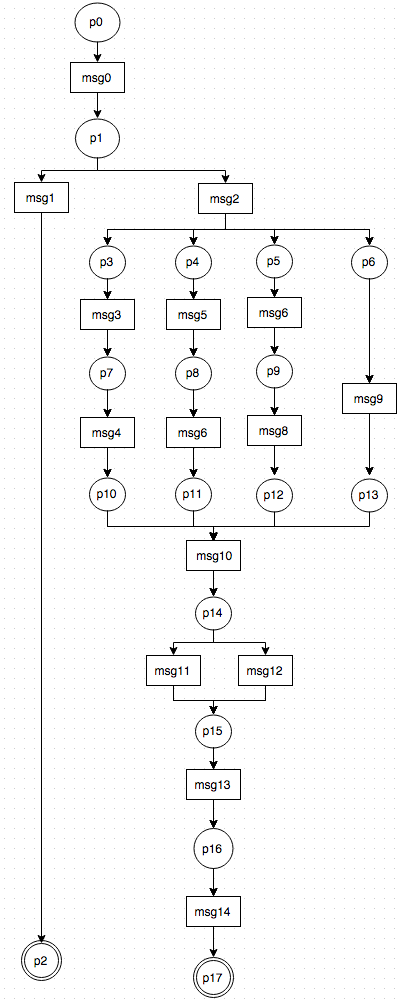
\includegraphics[width=3.1in]{figures/readDcache.png}}
 
 {\footnotesize
 \[
 \begin{array}{llll}
 msg0: (&\mbox{ CPU1},&\mbox{ReadReq},&\mbox{dcache1  })\\                   
 msg1: (&\mbox{ dcache1},&\mbox{ ReadRes},&\mbox{ CPU1 })\\
 msg2: (&\mbox{ icache1},&\mbox{ LoadLockedreq },&\mbox{Bus })\\     
 msg3: (&\mbox{ Bus},&\mbox{ LoadLockedreq},&\mbox{ dcahce2     })\\
 msg4: (&\mbox{ dcache2},&\mbox{LoadLockedreq},&\mbox{cpu2 })\\
 msg5: (&\mbox{ Bus},&\mbox{ LoadLockedreq},&\mbox{ icahce2     })\\ 
 msg6: (&\mbox{ icache2},&\mbox{LoadLockedreq},&\mbox{cpu2     })\\
 msg7: (&\mbox{ Bus},&\mbox{ LoadLockedreq},&\mbox{ dcahce1 })\\
 msg8: (&\mbox{ icache1},&\mbox{LoadLockedreq},&\mbox{cpu1       })\\
 msg9: (&\mbox{ Bus},&\mbox{ LoadLockedreq},&\mbox{ Memory     })\\
 msg10: (&\mbox{ true })\\
 msg11: (&\mbox{ Memory},&\mbox{ ReadRes},&\mbox{ Bus       })\\     
 msg12: (&\mbox{ icache2},&\mbox{ ReadRes},&\mbox{ Bus    })\\
 msg13: (&\mbox{ Bus},&\mbox{ ReadRes},&\mbox{ icache1 })\\
 msg14: (&\mbox{ dcache1},&\mbox{ ReadRes},&\mbox{ CPU1 })\\
 \end{array}
 \]}
 \caption{Flow specification ($F_2$) of a cache coherent read operation initiated from CPU1 to  data cache}
 \label{read-dcache}
 
 \end{figure}


The LPN specification shown in Fig.~\ref{read-dcahce} describes the system flow when CPU1 initiate a memory read operation to its data cache. DCache1 can also generate two possible responses to the read request. First, if the requested data is included in DCache1 but it's shared, cache1 will generate a load locked data request message msg21 to make sure it has the newest data. Second possibility is that when DCache1 has the requested, it will directly issue a read response message msg 33 to CPU1.


\begin{figure} 
 \centerline{
 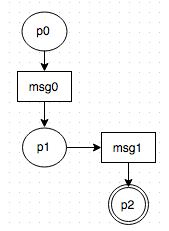
\includegraphics[width=1.5in]{figures/storeFail.png}}
 
 {\footnotesize
 \[
 \begin{array}{llll}
 msg0: (&\mbox{ CPU1},&\mbox{StoreFailedReq},&\mbox{ICache1})\\                   
 msg1: (&\mbox{ ICache1},&\mbox{ StoreFailedRes},&\mbox{ CPU1 })\\
 \end{array}
 \]}
 \caption{Flow specification ($F_2$) of a cache coherent read operation initiated from CPU1 to  data cache}
 \label{storefail}
 
 \end{figure}
Another flow implemented in GEM5 is when CPU initiate a store failed request to instruction cache, with a simple store failed response from instruction cache. Detailed flow specification is specified in Fig.~\ref{storefail}

This three specifications are also symmetric for CPU2.
\end{document}
